\clearpage
\section{Implementazione}

\subsection{Progettazione Architetturale}

\subsubsection{Requisiti non funzionali}
Per garantire la scalabilità e l'affidabilità del progetto useremo tecnologie in cloud,
 che permettono prestazioni altrimenti irraggiungibili, soprattutto nelle fasi iniziali dell'applicazione.\\
Questo comporta un sostanziale riduzione del carico di lavoro, in quanto al gestore cloud verranno delegati i requisiti di 
affidabilità, scalabilità, protezione da attacchi Ddos e la velocità delle comunicazioni\\ 
\subsubsection{Scelte tecnologiche}

Per familiarità con il sistema, disponibilità dei fondi e servizi offerti, 
la scelta del gestore cloud ricade su:
\begin{itemize}
    \item Google Firebase, per quanto la gestione degli accessi
    \item Microsoft Azure, per la logica applicativa e la persistenza.
\end{itemize}
In particolare, Google Firebase Authentication fornisce un sistema di autenticazione personalizzabile, 
oltre a dare la possibilità di gestire più identity providers.\\
TODO persistenza interna a gFA.\\
La logica di business dell'applicazione verrà sviluppata su Azure Functions, un servizio Faas che scala automaticamente le richieste al server.
La persistenza logica sarà affidata a AzureSQL, un database relazionale gestito dalla piattaforma, mentre le foto e i file multimediali verranno salvati su Azure Storage Container.
Per aggiornare i devices in tempo reale utilizzeremo Azure PubSub, che permette di creare un canale con ogni dispositivo.\\
Infine, per la fruizione del servizio tramite browser useremo Azure Static Web App, e, in attesa del rilascio ufficiale sul Play Store dell'applicazione, 
l'applicazione mobile sarà resa disponibile tramite Azure Storage Container.
\linebreak
Per quanto riguarda lo sviluppo, i principali linguaggi di programmazione saranno:
\begin{itemize}
    \item Flutter per l'interfaccia grafica, che permette di racchiudere in un'unica implementazione applicazioni per dispositivi di tecnologia differente
    \item C\# per la logica di business, nativamente supportato dalle Functions, permette un collegamento diretto tra oggetti logici e database, semplificando la gestione della persistenza.
\end{itemize}
\pagebreak

\subsubsection{Scelta dell'architettura}
\begin{figure}[h!]
    \begin{center}
        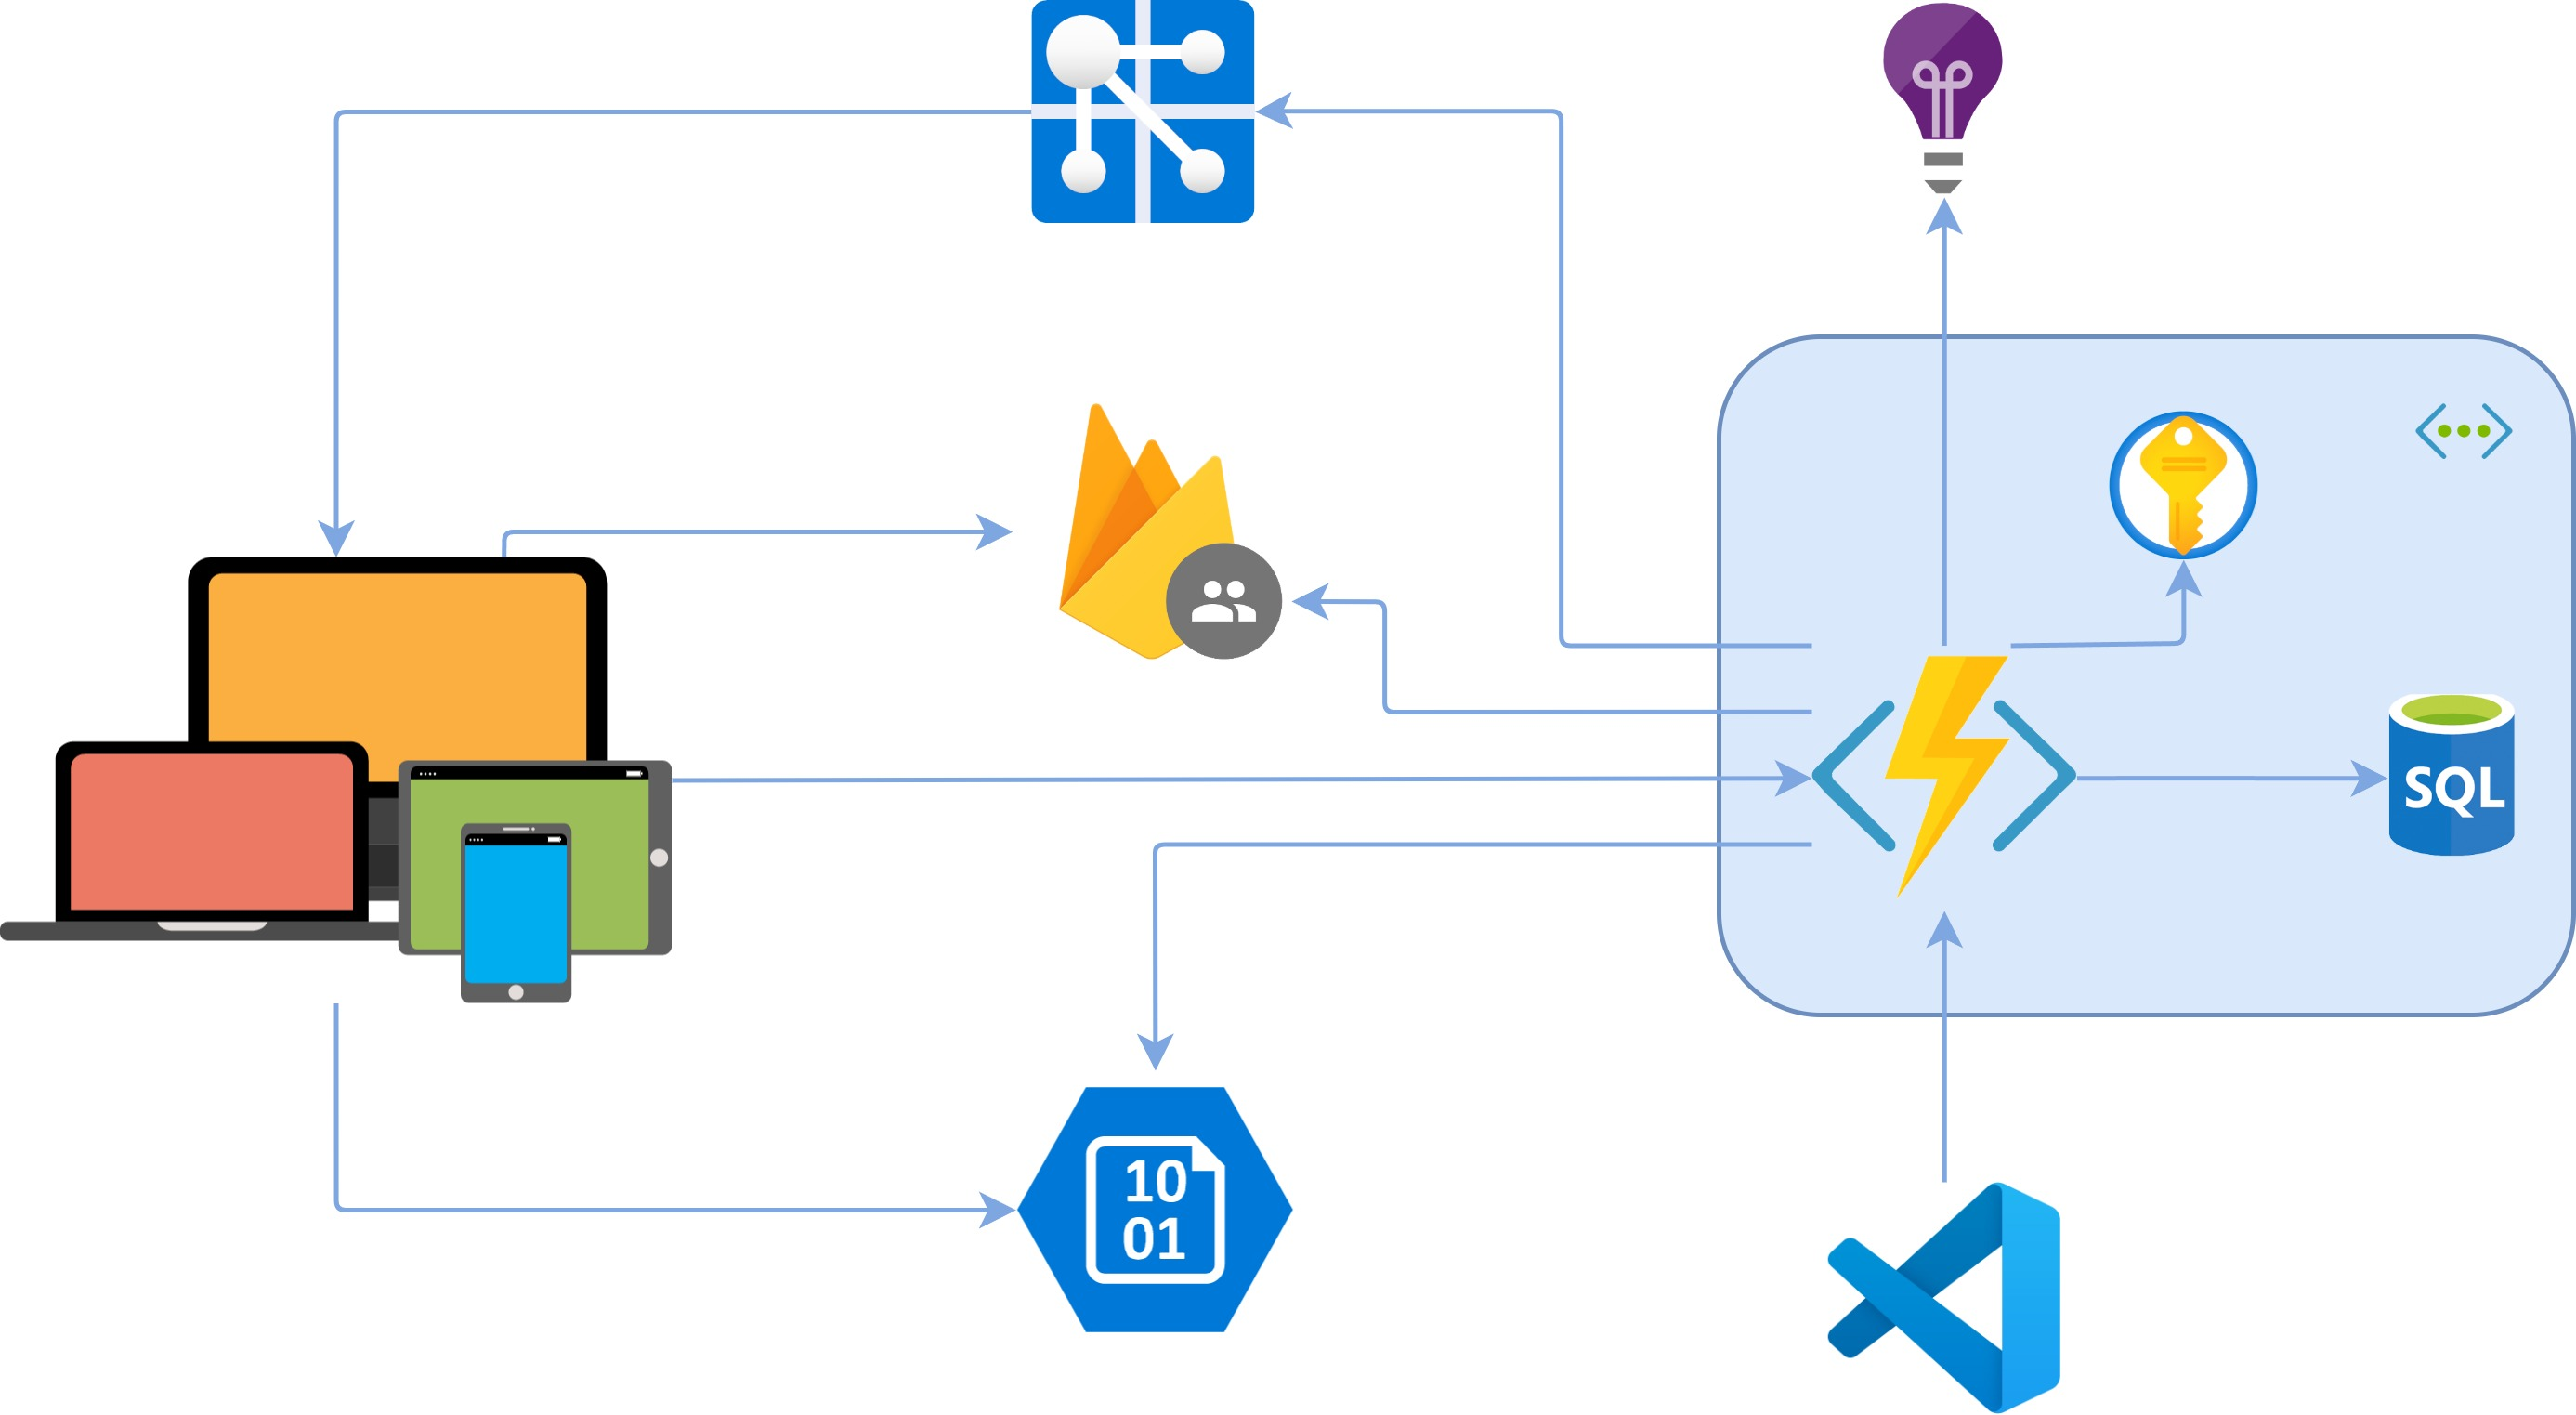
\includegraphics[width=\textwidth]{ImplementazioneArchitettura.jpg}
    \end{center}
\end{figure}
Nel grafico possiamo notare come al centro dell'architettura ci siano le Azure Functions che, all'interno della stessa rete, comunicano con il database relazionale e il Key Vault.
In base alla richiesta, che partirà sempre dal dispositivo dell'utente, le Functions potranno poi interagire con 
il servizio Pub-Sub per gli aggiornamenti in tempo reale, 
Google Firebase per l'autenticazione o 
Azure Storage Container per le immagini.
I devices degli utenti avranno quindi la possibilità di contattare autonomamente, oltre alle Functions, sia Google Firebase che il server per la persistenza delle immagini. 
\subsection{Monitoraggio}
Il monitoraggio del sistema avverrà in due modi: tramite salvataggio dei log e controllo delle prestazioni del sistema.\\
Per quanto riguarda Firebase Authentication vengono forniti in con il servizio sia le interfacce per il controllo delle prestazioni che la gestione dei log.\\
Per monitorare le Azure Functions sarà necessario collegare Azure Application Insights che provvede a controllare il funzionamento e la risposta del servizio.
La creazione dei log è invece affidata al programmatore, che verranno poi salvarti tramite function su un file sistem dedicato su un Azure Container. 

\subsection{Sicurezza}
Per garantire la sicurezza nelle comunicazioni ogni interazione avverrà utilizzando un canale sicuro cifrato grazie al protocollo HTTPS.\\
Tutte le credenziali e variabili di ambiente usate dalle Azure Functions per collegarsi ai database 
e ai vari servizi saranno conservate e ottenute tramite Azure Key Vault, per garantire la confidenzialità delle credenziali.\\
Il server di accesso rilascerà un token, unico per ogni utente, che verrà allegato ad ogni richiesta, 
per essere usato dal server principale per identificare l'utente ed eventualmente controllare i permessi relativi.
Il token deve permettere di identificare ed autenticare univocamente l'utente.\\
La generazione degli hash di identificazione dei componenti deve garantire una diffusione tale da rendere altamente improbabile una collisione.\\
Le richieste di salvataggio dati non possono superare i 100 Kb di dimensione, 
e ogni utente non può fare in un arco orario richieste in scrittura che vadano complessivamente oltre i 20 MB.\\
Come evidenziato precedentemente, la difesa da attacchi di tipo denial of service verranno affidati al cloud provider\\
Inoltre, sarà necessario che tutto il codice, in fase di sviluppo, venga controllato da esperti di sicurezza, 
per ridurre il più possibile l'integrazione di falle nel sicurezza.\\ 

\newpage
\subsection{Progettazione di dettaglio}

Di seguito verranno schematizzati alcuni esempi generali per mostrare le modifiche da apportare in seguito alle scelte implementative, come linee guida per il resto del programma.\\
I casi particolari di interazione verranno dettagliati nella relativa sezione.

\paragraph{Struttura: Dominio}\mbox{}\\

Sia per il client che per il server, ogni entità descritta nel dominio verrà mappata con una classe corrispondente.
TODO classi dominio .dart .cs\\

\paragraph{Struttura: Controller - Client}\mbox{}\\
Ogni richiesta di dati verso l'esterno verrà implementata grazie a classi che nasconderanno i dettagli necessari per la comunicazione, chiamate API.\\
Inoltre, funzionalità che vengono ripetute in parti diverse del programma verranno delegate a classi chiamati servizi, che raggrupperanno le richieste per affinità logica.\\
A titolo esemplificativo, si riportano alcune classi:\\
TODO classi front API e Services
notificationservice.

Flutter ha una gestione dello stato che si basa sulla vita dei componenti a cui è associato. La persistenza a livello locale ha quindi durata limitata e ricade nella normale programmazione del framework.\\
La persistenza di livello applicativo verrà suddivisa in base alle classi logiche del dominio. Le classi seguiranno un pattern singleton e verranno create all'avvio dell'applicazione.\\
TODO front providers


\paragraph{Struttura: Controller - Server}\mbox{}\\
Per sfruttare le caratteristiche di scalabilità delle Functions, il codice dovà essere suddiviso in nuclei di codice indipendenti tra loro, senza la permanenza di uno stato tra una richiesta e l'altra.\\
Anche in questo caso, alcune funzionalità potrebbero essere condivise da più function, per cui verranno raggruppate in classi chiamate service.\\
Infine, per la conversione delle classi di dominio a quelle di risposta, si implementeranno dei data tranfert objects(DTO) che permetteranno una mappatura corretta con il dominio dei client.\\







\subsubsection{Interazione}

Registrazione\\

Login\\

Visualizza eventi confermati\\

modifica evento\\

conferma immagini\\

condivisione con gruppi

condivisione tramite link\\









\subsection{Deployment e Aggiornamento del Codice}

\subsubsection{Deployment Type-Level: Client}

\begin{figure}[h!]
    \begin{center}
        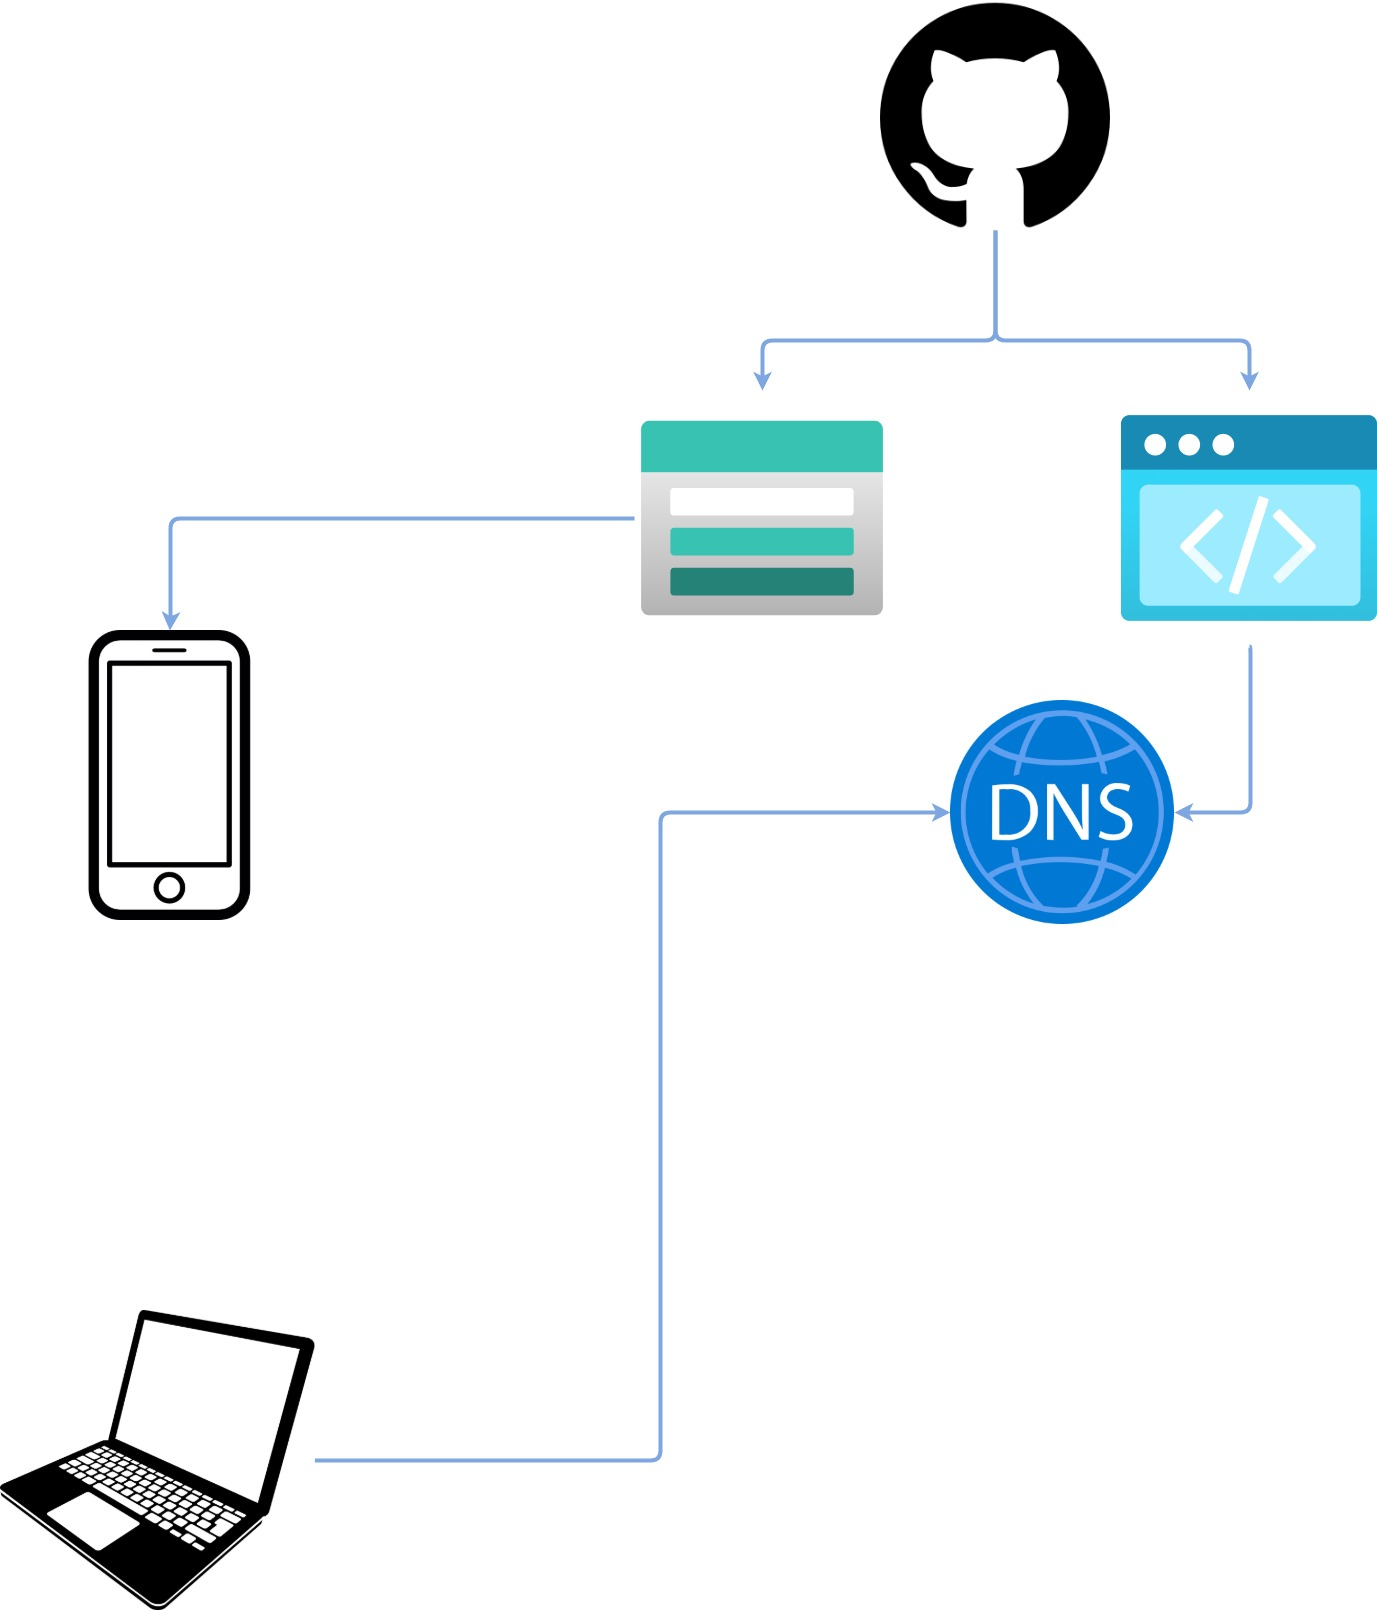
\includegraphics[width=\textwidth]{ImplementazioneDeployment.jpg}
    \end{center}
\end{figure}
Aggiornamento lato web gestito automaticamente, lato applicazione tramite notifica che chiederà all'utente di aggiornare la sua applicazione.\\
\newpage
\subsubsection{Deployment Type-Level: Server}

\begin{figure}[h!]
    \begin{center}
        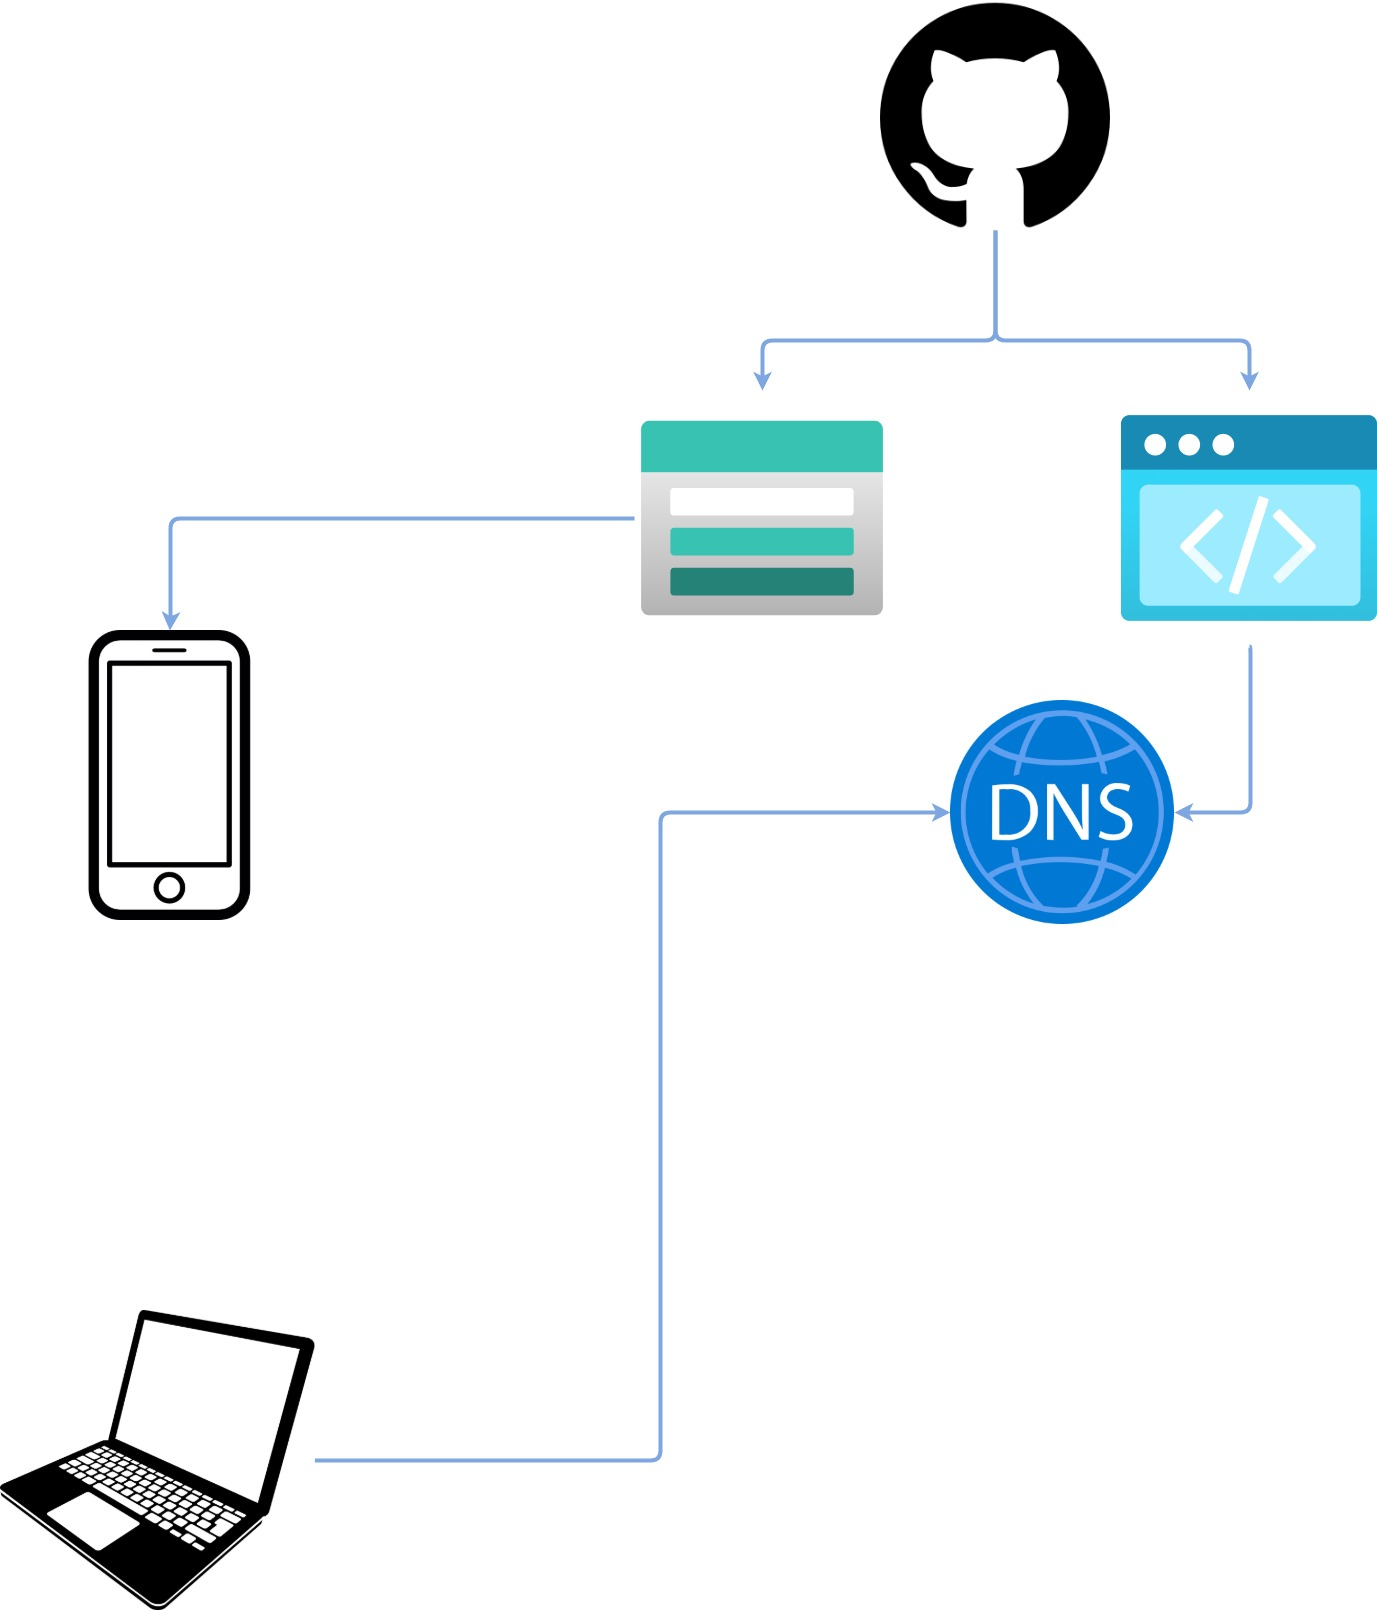
\includegraphics[width=\textwidth]{ImplementazioneDeployment.jpg}
    \end{center}
\end{figure}
L'aggiornamento del codice eseguito sulle Azure Functions avverrà tramite un comando dato tramite interfaccia grafica su Visual Studio Code grazie all'estensione Azure Tools.\\
Le modifiche al dominio del database verranno applicate tramite migrations, 
generate automaticamente dal framework C# grazie alla libreria EFCore che permette di mappare le classi in tabelle SQL.\\

\subsection{Testing e Performances}
